% !TEX root = ../main.tex
\section{Related Work}
\label{sec:related}
\begin{figure}
\centering
\subfloat[ARToolkit]{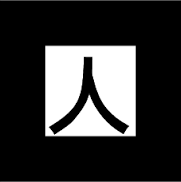
\includegraphics[width=50px, height=50px]{figs/tags/artoolkit}} \quad
\subfloat[ARTag]{
\includegraphics[width=50px, height=50px]{figs/tags/artags}} \quad 
\subfloat[AprilTag]{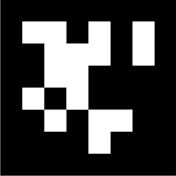
\includegraphics[width=50px, height=50px]{figs/tags/apriltags}} \\
\subfloat[RUNE-Tag]{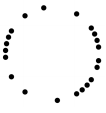
\includegraphics[width=50px, height=50px]{figs/tags/rune}} \quad
\subfloat[Intersense]{
\includegraphics[width=50px, height=50px]{figs/tags/intersense}}
\caption{Different types of popular fiducial tags. ARToolkit, ARTags, and AprilTags are square tags with black borders. RUNE-tags and Intersense use different circle features as landmarks}
\label{fig:tags}
\end{figure}
	Obtaining highly accurate pose estimation has been an important research area in robotics. Numerous algorithms rely only on RGB or gray scale images. Solving the projection geometry of some detected features and then minimize the reprojection error of the features in the image space \citep{grest2009comparison}.  Similarly, methods such as Iterative Closet Point \citep{besl1992method} were developed to solve the pose estimation problem using range data by minimizing the Euclidean distance between the model and the depth data. Recently, some approaches propose to enhance the accuracy of traditional tracking algorithms by fusing RGB and depth data in various problems using extended Kalman filters \citep{gedik2015rgbd, assa2014robust}. Compared to the single-sensor approaches, algorithms utilizing RGBD data are more accurate and perform well in noisy situations where other approaches fail. In this paper, we take a similar approach to improve the pose estimation in fiducial markers.
	
	Fiducial markers solve pose estimation by exploiting easily detectable features in the RGB space. There is an abundance of unique tag designs, most of them carry easily recognizable yet precise binary patterns in the inner region to encode information. There are two types of common tags: circular tags and square tags seen in Figure \ref{fig:tags}. 
	
	Circular tags are created to encode the payload using small circular patterns arranged in various shapes. The example of circular tags include Intersense \citep{naimark2002circular} and Rune tags \citep{bergamasco2011rune}. The perspective transformation of a circle is an ellipse, which can be used to directly compute the pose using back projection methods. Localization of circular features is generally more accurate, and thus generates better pose estimation at the cost of higher computation time \citep{rice2006analysing}. However, small circular features become hard to detect when they are far away from the camera or prospectively rotated, and thus their effective range is much smaller than that of square tags. This characteristic makes them less useful in applications with size constraints. 
	
\begin{figure}
\centering
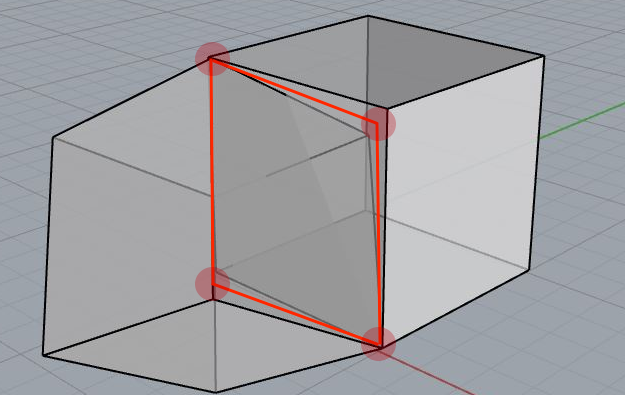
\includegraphics[width=\columnwidth]{figs/perspective_fig}
\caption{The ambiguity effect is illustrated with two rendered cubes in the perspective view. The two cubes are rotated such that two faces are interlaced. The red square is a simulated projection of a square tag. The red circular regions denote the region of potential corner detections in a noisy scene. The pose of the red square can converge to either one of the two faces.}
\label{fig:cube}
\end{figure}
	
		
\begin{figure*}[h]
\subfloat[]{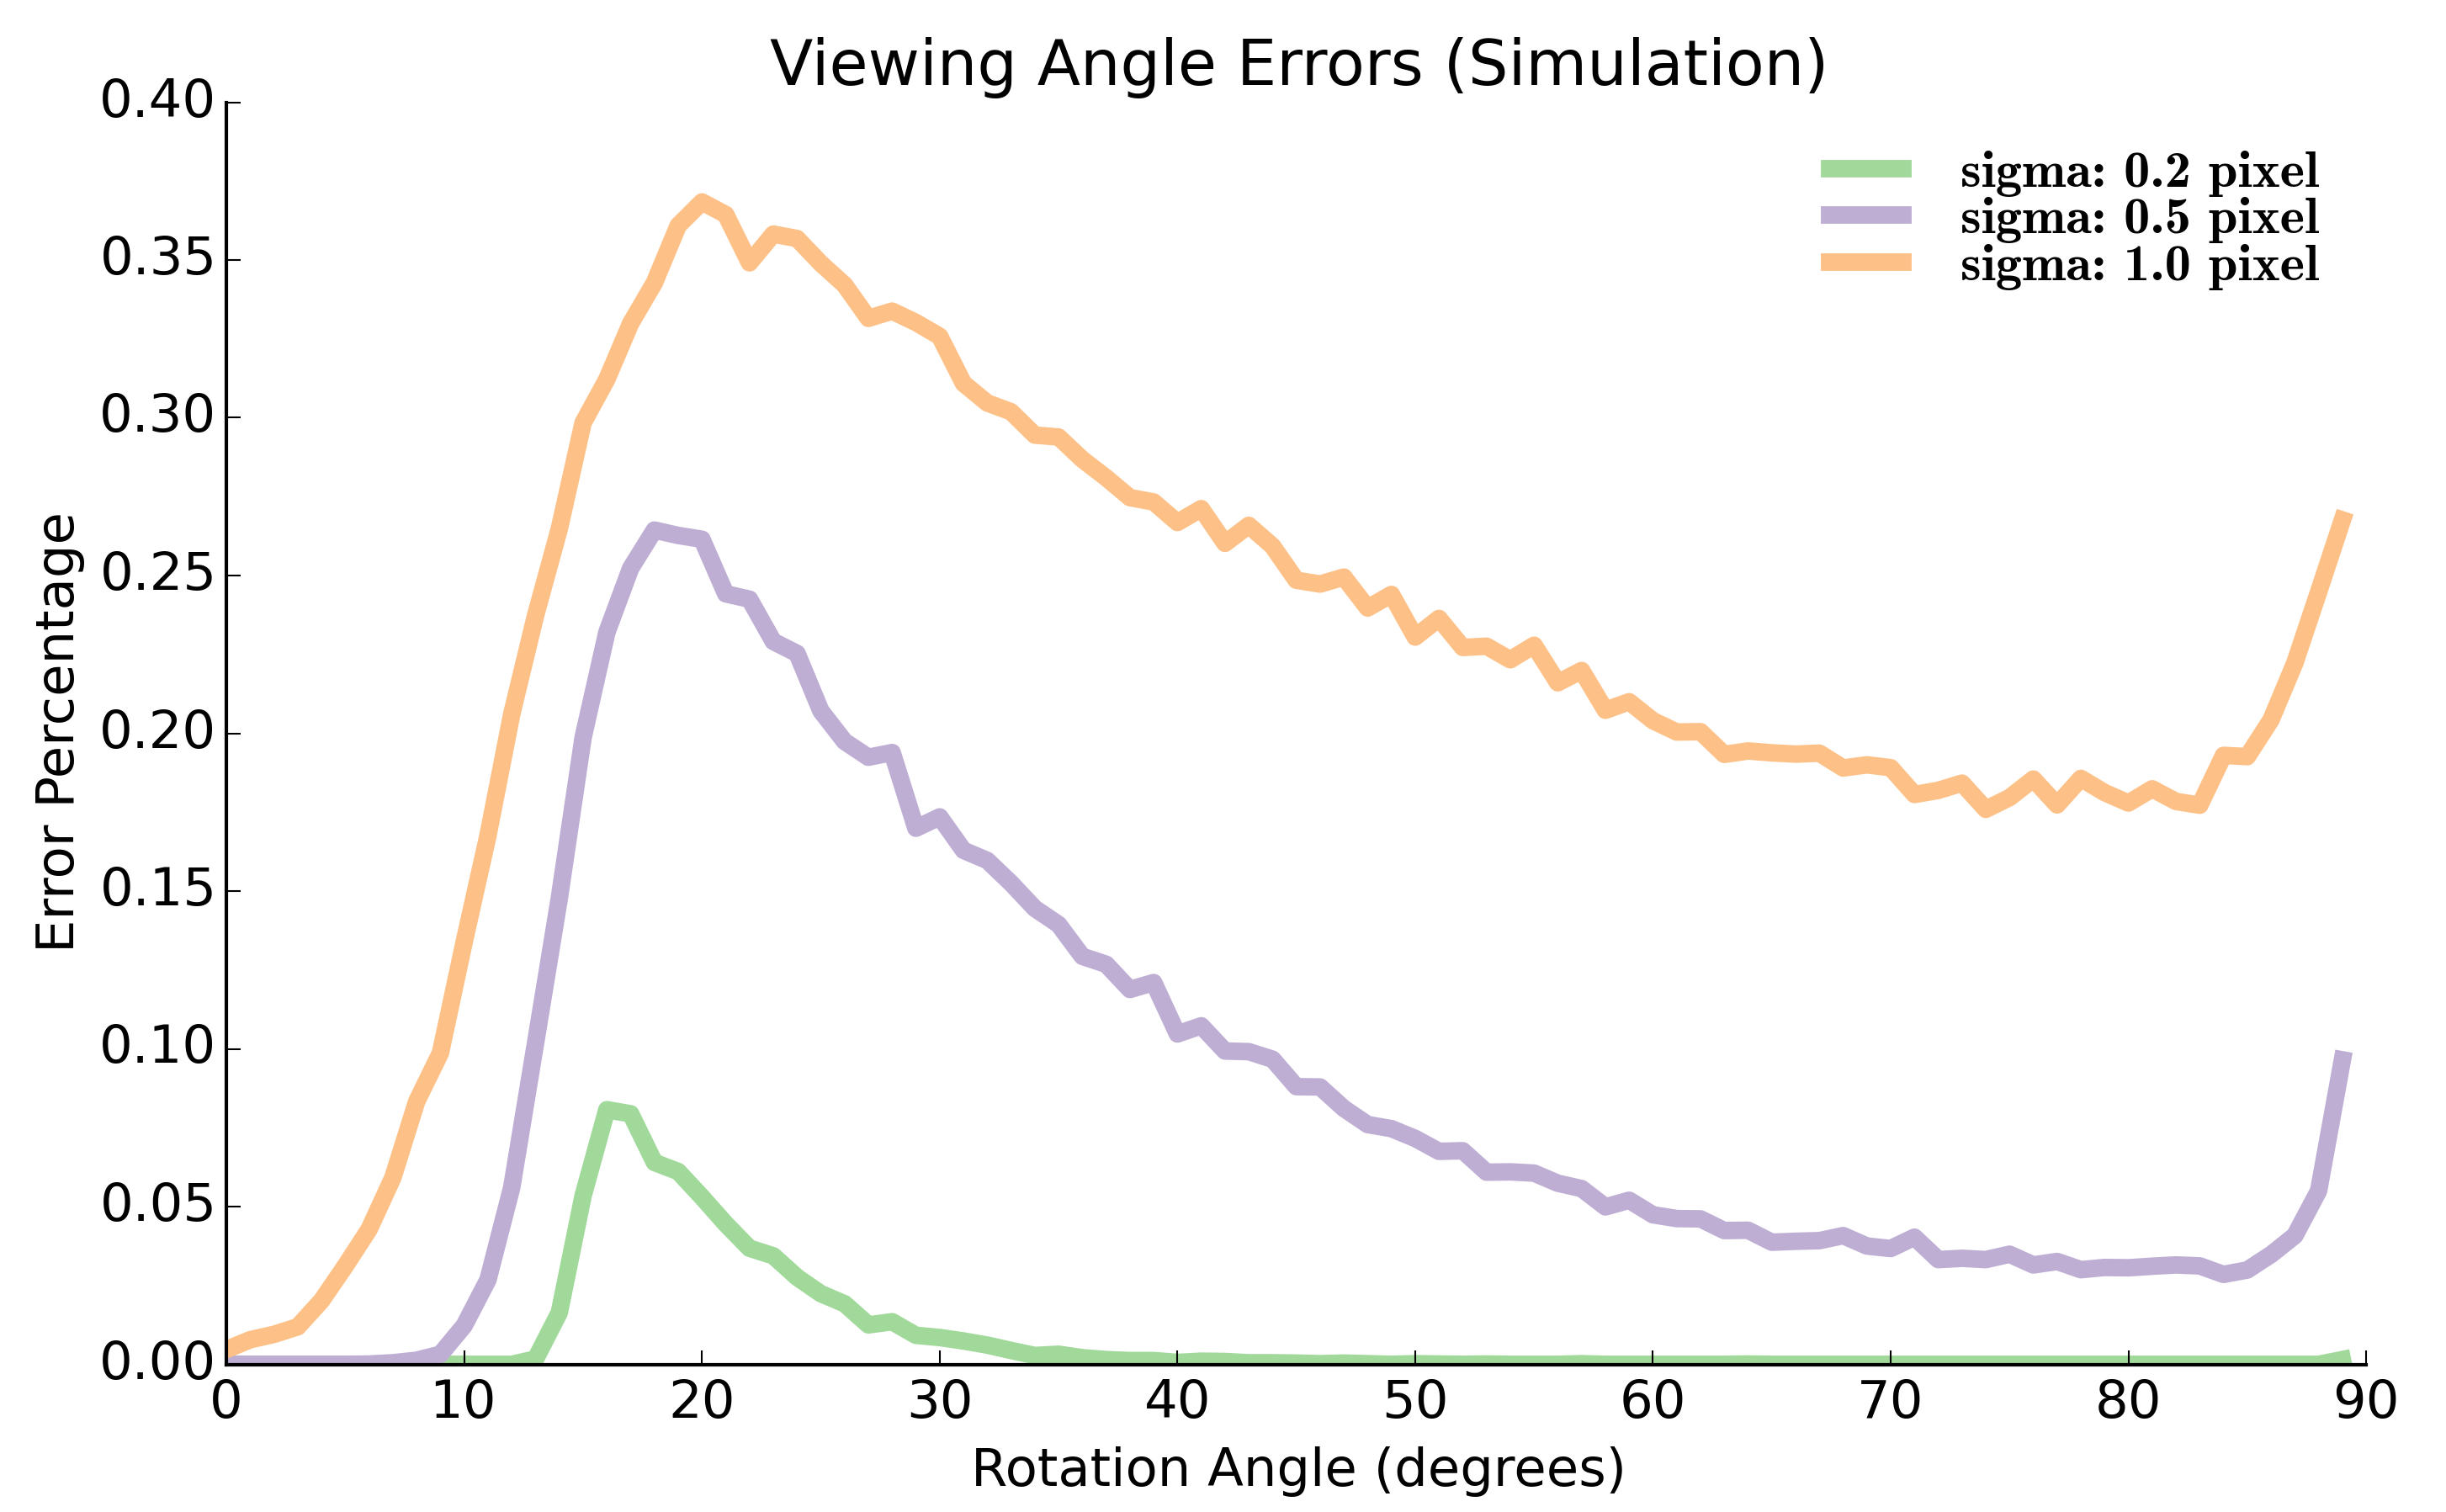
\includegraphics[width=\columnwidth, height=160px]{figs/simulation_rotation}
\label{fig:simulation_rotation}} 
\subfloat[]{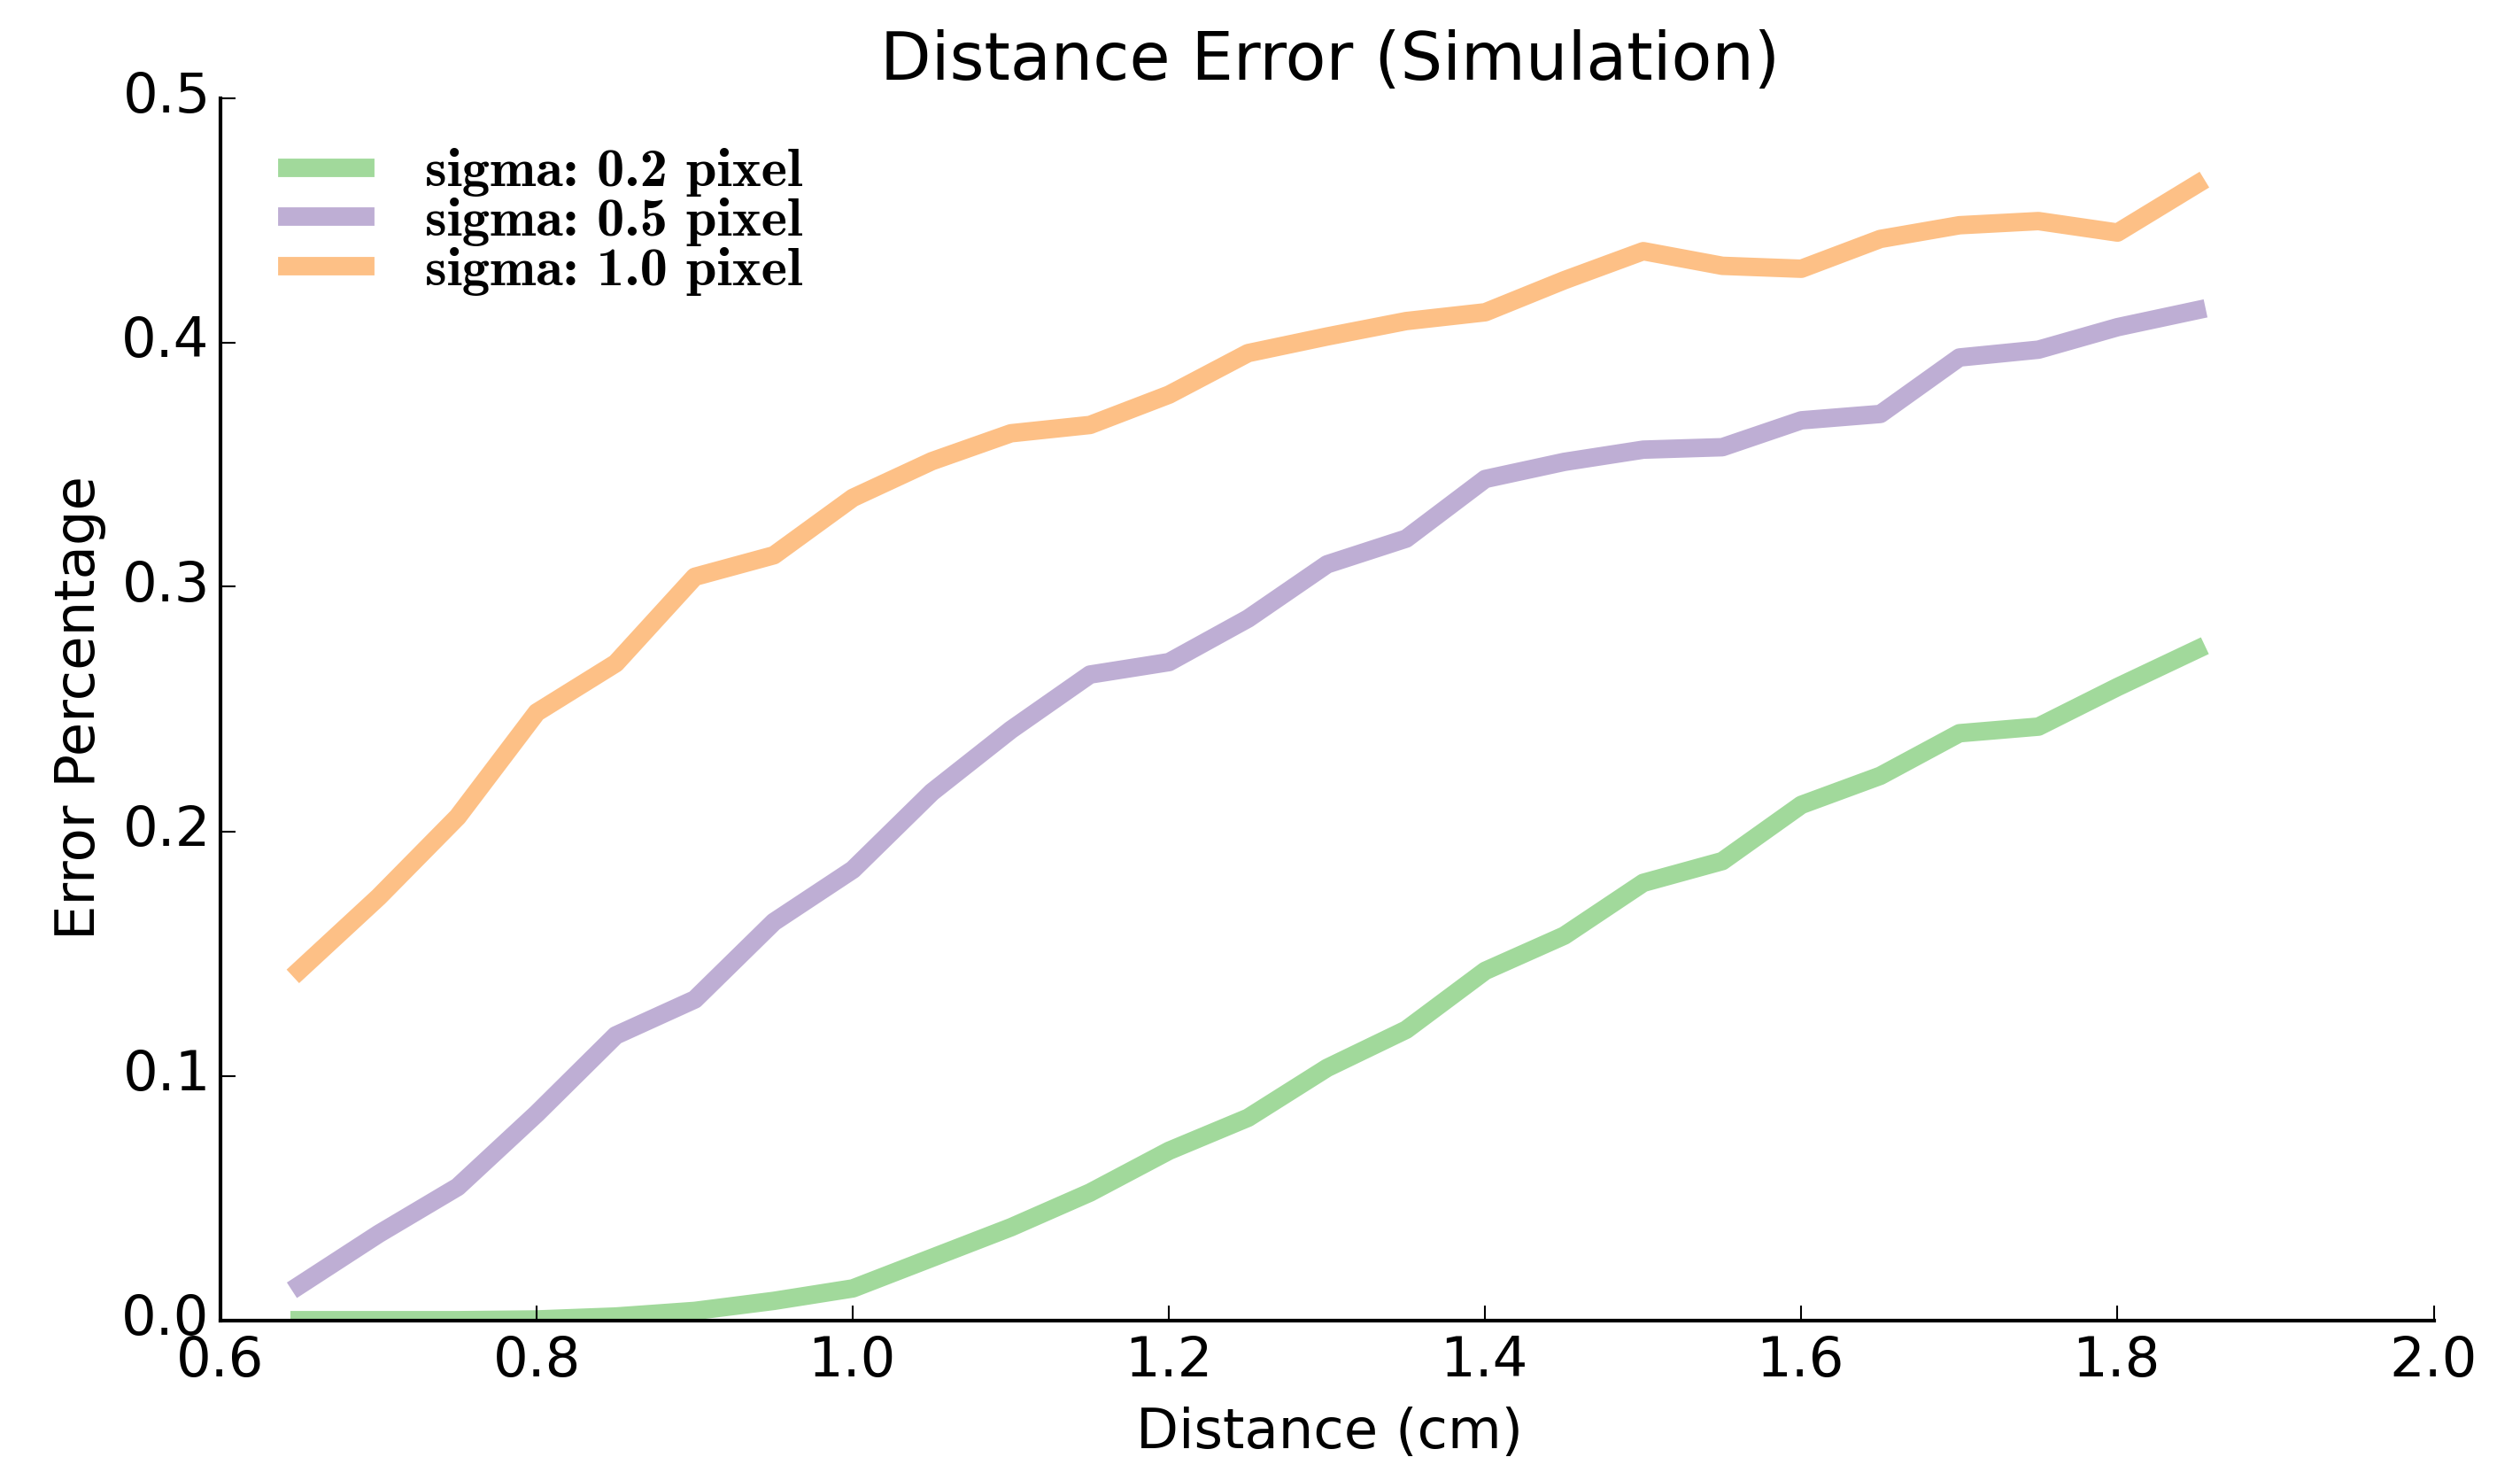
\includegraphics[width=\columnwidth, height=160px]{figs/simulation_trans}
\label{fig:simulation_translation}} 
\caption{Simulation results of Apriltag pose estimation under different noise level. In both simulations, four corners are projected onto a rendered image with some noise then computed their poses in each trail. In \ref{fig:simulation_rotation}, corners are projected to the center of the camera 0.8 meters away and rotated from $0^{\circ}$ to $90^{\circ}$. In \ref{fig:simulation_translation}, the corners are projected at $40^{\circ}$ and moved from 0.6 meters to 1.8 meters. We sampled the poses from 10,000 trials for each experiment and computed the percentage of unacceptable poses base on a threshold.}
\label{fig:simulation_results}
\end{figure*}	
	
	ARTags \citep{fiala2004artag}, ARToolkit \citep{kato2002artoolkit}, AprilTag \citep{olson2011apriltag} and AprilTag 2 \citep{wang2016apriltag} are examples of squared-based fiducial tags. The perspective projection of a square becomes a general quadrilateral. Given the scale of a single marker, the full 6-DOF pose can then be estimated using the corners of the quadrilateral. However, since the tags are detected using rectangles and lines, the accuracy of their corner point sub-pixel locations is limited. Among the square tags, ARToolkit is one of the earliest detection systems, and it is mainly used for Augmented reality applications. Instead of using a binary payload, it used various symbols to encode the tag, and it was computationally expensive to decode the tag. Built on top of ARToolkit, ARTags and Apriltag reduced the computation time by using a 2D binary pattern as the payload. Both systems use the image gradient to compute the tag border making it robust to lighting changes and partial occlusions. Relative to ARTags, Apriltags have a lower false positive rate, as they use a lexicode-based system that is invariant to rotation. In addition, Apriltags have higher detection rates at further distances and at more difficult viewing angles. Recently AprilTag 2 improved upon the original Apriltag. It implements a new boundary segmentation algorithm which further reduces the computing time for detection and increases the detection rate. Compared to circular tags, the advantages of square tags are that they can be located very efficiently and they have reliable decoding schemes. Therefore, even though the square tags have slightly lower localization accuracy, they are more suitable for robotic applications that require a robust system.
